\subsubsection{Directions Viewer}
The Directions Viewer was implemented in the following manner:
\begin{description}
\item[BranchLocation] A container for the DirectionsMap class which also loads
the Maps API. It also provides a communication interface between DirectionsMap
and the rest of the system and allows the user to change their location.
\item[DirectionsMap] A container for a MapWidget~\cite{mwidget} and a
DirectionsPanel~\cite{dpanel} which loads a new map and directions when 
provided with data in the form of a LatLng~\cite{latlng} map center and a
String~\cite{string} containing an origin and a destination.
\end{description}
\begin{figure}[h!]
\centering
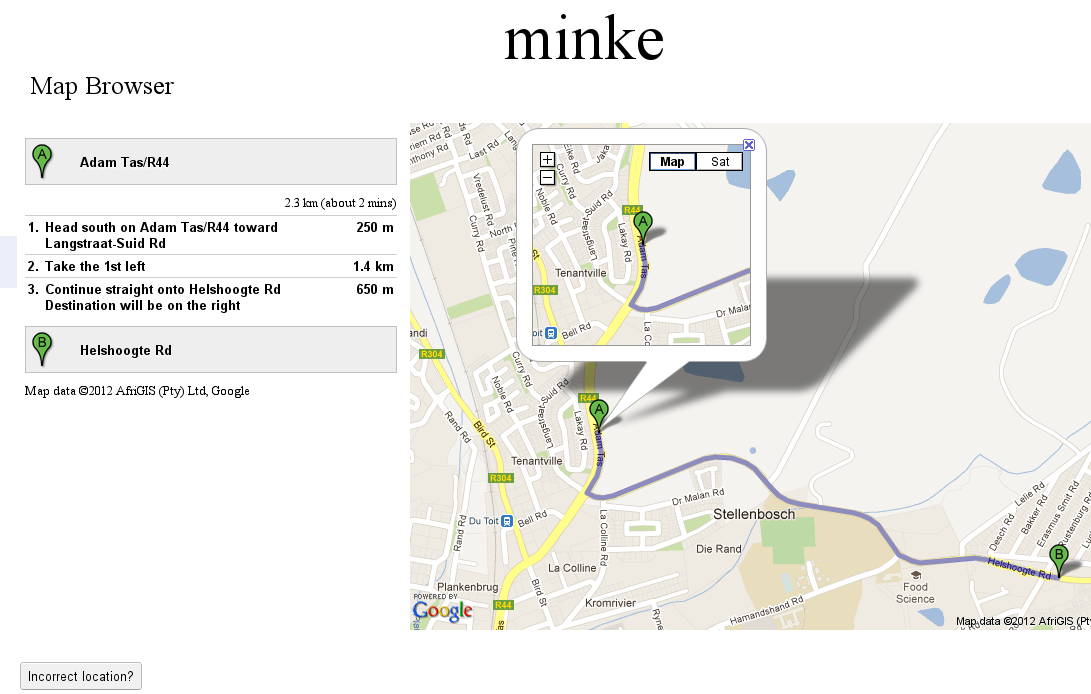
\includegraphics[width=0.8\textwidth]{gwt-map.png}
\caption{The Directions Viewer.}
\end{figure}